\documentclass[tikz,border=0pt,11pt]{standalone}
\usepackage[T1]{fontenc}
\usepackage[utf8]{inputenc}
\usepackage{lmodern,amsmath,amssymb}
\usepackage[swedish]{babel}
\usetikzlibrary{arrows.meta,calc,positioning,decorations.pathmorphing,decorations.pathreplacing,patterns,shadings}
\definecolor{navy}{HTML}{102F40}
\definecolor{teal}{HTML}{147D78}
\definecolor{lightteal}{HTML}{E6F1ED}
\definecolor{gold}{HTML}{B88B3B}
\definecolor{palegold}{HTML}{F7EEDB}
\definecolor{rust}{HTML}{B6533B}
\definecolor{palerust}{HTML}{FAEAE4}
\definecolor{paper}{HTML}{F7F5EE}
\definecolor{muted}{HTML}{5B6D72}
\definecolor{line}{HTML}{D6DED8}
\renewcommand{\familydefault}{\sfdefault}
\newcommand{\atom}[5]{\shade[ball color=#3!70] (#1,#2) circle (#5);\node[text=white,font=\bfseries\small] at (#1,#2){#4};}
\newcommand{\water}[3]{\begin{scope}[shift={(#1,#2)},scale=#3]\draw[navy!45,line width=2pt] (-.3,.22)--(0,0)--(.3,.22);\atom{0}{0}{rust}{O}{.22}\atom{-.3}{.22}{teal}{H}{.15}\atom{.3}{.22}{teal}{H}{.15}\end{scope}}
\newcommand{\panel}[4]{\filldraw[fill=white,draw=line,rounded corners=5pt] (#1,#2) rectangle ++(#3,#4);}
\newcommand{\note}[4]{\node[txt,text width=#3cm] at (#1,#2){#4};}
\tikzset{txt/.style={anchor=north west,align=left,text=navy,font=\small},
 head/.style={anchor=west,text=navy,font=\bfseries\large},
 label/.style={align=center,text=navy,font=\small},
 smalllabel/.style={align=center,text=muted,font=\footnotesize},
 arrow/.style={-{Latex[length=2.5mm,width=1.8mm]},line width=1.2pt,draw=teal},
 goldarrow/.style={-{Latex[length=2.5mm]},line width=1.2pt,draw=gold},
 rustarrow/.style={-{Latex[length=2.5mm]},line width=1.2pt,draw=rust},
 dashedarrow/.style={arrow,dashed},
 badge/.style={fill=lightteal,rounded corners=3pt,text=teal,font=\bfseries\small,inner sep=5pt}}
\begin{document}
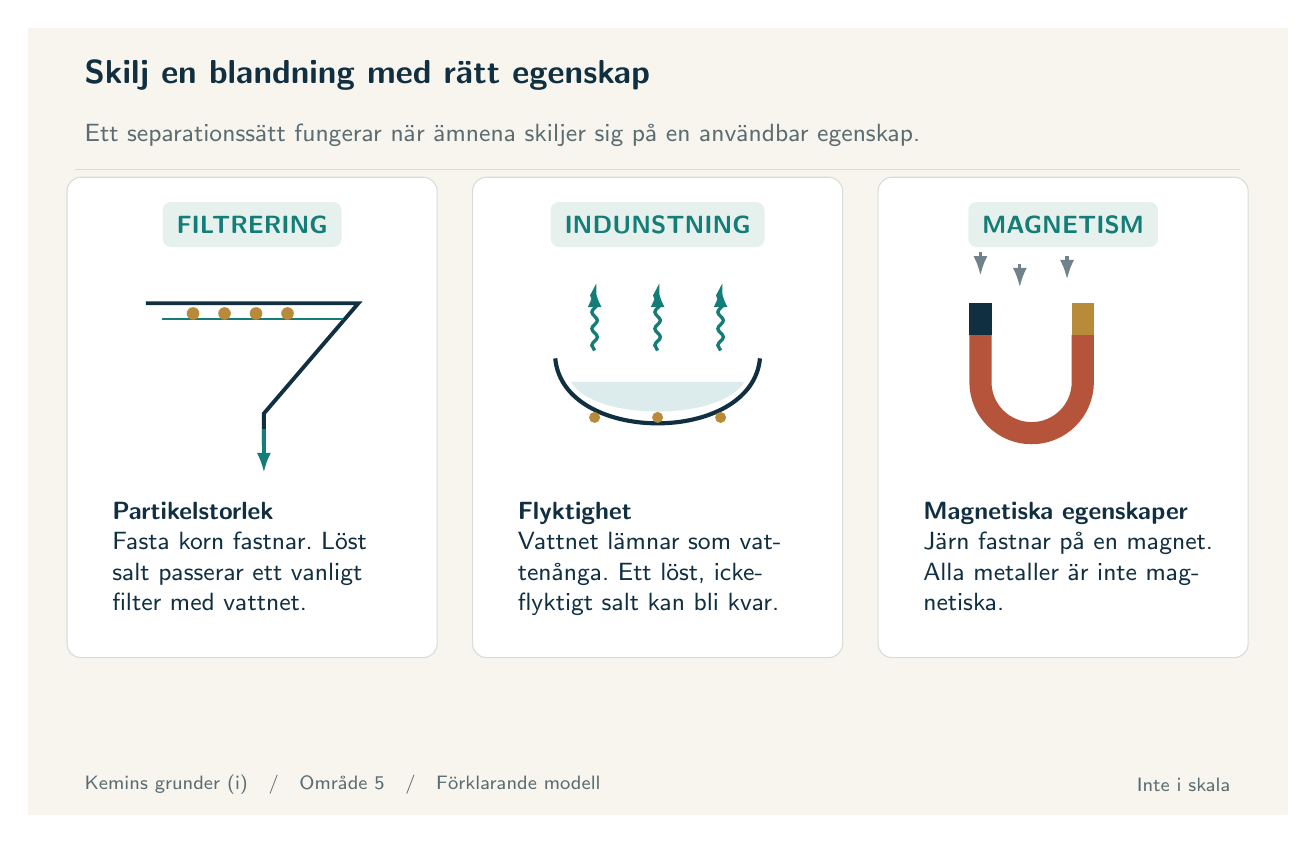
\begin{tikzpicture}[x=1cm,y=1cm]
\path[use as bounding box] (0,0) rectangle (16,10);
\fill[paper] (0,0) rectangle (16,10);
\node[head] at (.6,9.4){Skilj en blandning med rätt egenskap};
\note{.6}{8.9}{14.8}{\textcolor{muted}{Ett separationssätt fungerar när ämnena skiljer sig på en användbar egenskap.}}
\draw[line] (.6,8.2)--(15.4,8.2);

\foreach \x in {.5,5.65,10.8}{\panel{\x}{2}{4.7}{6.1}}
\node[badge] at (2.85,7.5){FILTRERING};\node[badge] at (8,7.5){INDUNSTNING};\node[badge] at (13.15,7.5){MAGNETISM};
\draw[navy,line width=1.4pt] (1.5,6.5)--(4.2,6.5)--(3,5.1)--(3,4.7);\draw[teal,line width=1pt] (1.7,6.3)--(4,6.3);\foreach \x in {2.1,2.5,2.9,3.3}{\fill[gold] (\x,6.37) circle(.08);}\draw[arrow] (3,4.9)--(3,4.35);
\draw[navy,line width=1.5pt] (6.7,5.8)..controls(6.8,4.7)and(9.2,4.7)..(9.3,5.8);\fill[teal!15] (6.9,5.5)..controls(7.2,5)and(8.8,5)..(9.1,5.5)--cycle;\foreach \x in {7.2,8,8.8}{\draw[arrow,decorate,decoration={snake,amplitude=1pt,segment length=6pt}] (\x,5.9)--(\x,6.7);\fill[gold] (\x,5.05) circle(.07);}
\draw[rust,line width=8pt] (12.1,6.1)--(12.1,5.5) arc(180:360:.65)--(13.4,6.1);\draw[navy,line width=8pt] (12.1,6.1)--(12.1,6.5);\draw[gold,line width=8pt] (13.4,6.1)--(13.4,6.5);\foreach \x/\y in {12.1/6.85,12.6/6.7,13.2/6.8}{\draw[arrow,navy!60] (\x,\y+.3)--(\x,\y);}
\note{.95}{4.1}{3.8}{\textbf{Partikelstorlek}\par Fasta korn fastnar. Löst salt passerar ett vanligt filter med vattnet.}
\note{6.1}{4.1}{3.8}{\textbf{Flyktighet}\par Vattnet lämnar som vattenånga. Ett löst, icke-flyktigt salt kan bli kvar.}
\note{11.25}{4.1}{3.8}{\textbf{Magnetiska egenskaper}\par Järn fastnar på en magnet. Alla metaller är inte magnetiska.}\node[anchor=west,text=muted,font=\scriptsize] at (.6,.38){Kemins grunder (i)\quad /\quad Område 5\quad /\quad Förklarande modell};
\node[anchor=east,text=muted,font=\scriptsize] at (15.4,.38){Inte i skala};
\end{tikzpicture}\end{document}
